The Approximate Data Transfer (ADT) procedure compresses network's weights
before they are transferred to the GPUs.
In the context of DNNs training on heterogeneous multi-GPU nodes, CPU multicore devices 
are typically responsible for orchestrating the parallel run and updating DNN parameters.
%It also updates the weights as the training process progresses. 
Once the process of a batch starts, the updated parameters including the weights $W$ are sent to each GPU.
%so that all of them contain the current state of the training process.
If the set of parameters does not fit in GPUs' main memory, they are sent on several phases as the different GPUs need them.
The different samples of each batch are evenly distributed across all GPUs.
Therefore, each GPU computes its contribution to the gradient $\Delta W$ by processing its corresponding set of samples.
The CPU multicore device subsequently gathers all contributions to the gradient and 
combines them to update the weights 
$W \gets W - \mu (\frac{1}{n} \sum_{i}^{n} \Delta W_{i})$, where $\mu$ is 
the learning rate.

Data movement involving different GPU devices increases as the network topology becomes more complex or the number of training samples grows, which can saturate the system bandwidth and become a major performance bottleneck.
This paper mitigates this issue by compressing network weights before they are sent to the GPU devices.
The AWP algorithm described in Section~\ref{sec:bitpack_adaptive} determines, for all  
weights belonging to a particular network layer, the number of bits to send.
%AWP keeps the training quality by changing weights' data representation. 
In this context, to efficiently compress and decompress network weights, ADT uses of two procedures that constitute its fundamental building blocks. 
These procedures are complementary and applied either before or after data transfers to GPU devices.
\begin{itemize}
    \item \textbf{Bitpack} compresses the weights discarding the less significant bits on the CPU side;
    \item \textbf{Bitunpack} converts the weights back to the IEEE-754 32-bit Floating Point format on the GPUs. 
\end{itemize}

Figure~\ref{bitpack_mgpu} provides an example including a multicore CPU and two GPU devices to describe the way both Bitpack and Bitunpack procedures operate.
All neural network parameters (weights and biases) are updated at the CPU level, which is where the Bitpack procedure takes place. 
We do not apply the Bitpack procedure to the network biases since we do not observe any significant performance benefit from compressing them.
Since each output neuron requires just one bias parameter, the total number of them is significantly smaller than the total number of weights.
At the beginning of each SGD iteration the compressed weights are sent to each GPU together with the biases and the corresponding training samples.
Each GPU uncompresses the weights, builds the neural network model  
and, finally, computes its specific contribution to the gradient.
These contributions are sent to the CPU, which gathers all of them, computes the gradient and updates network parameters.

\begin{figure}%[bhtp]
    \centerline{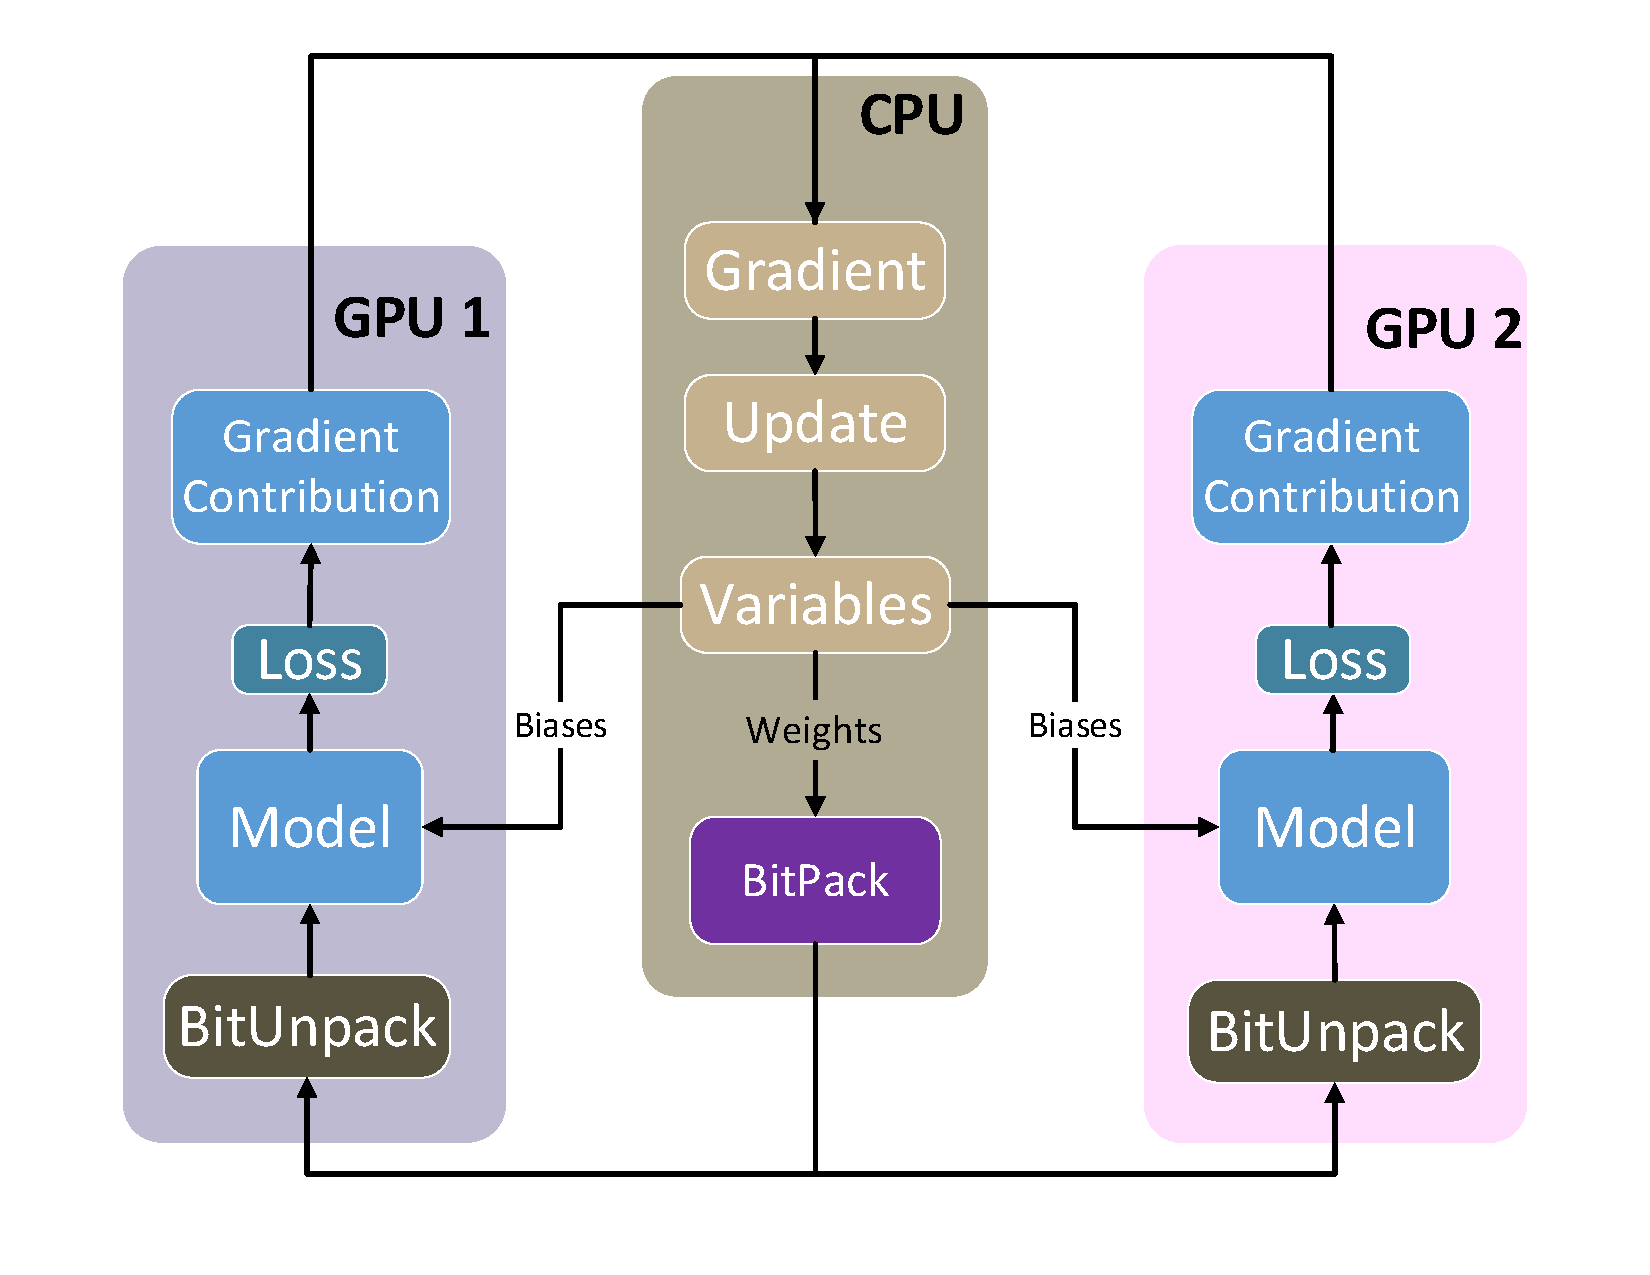
\includegraphics[scale=0.50]{bitpack/figs/drawing6.pdf}}
    %\centerline{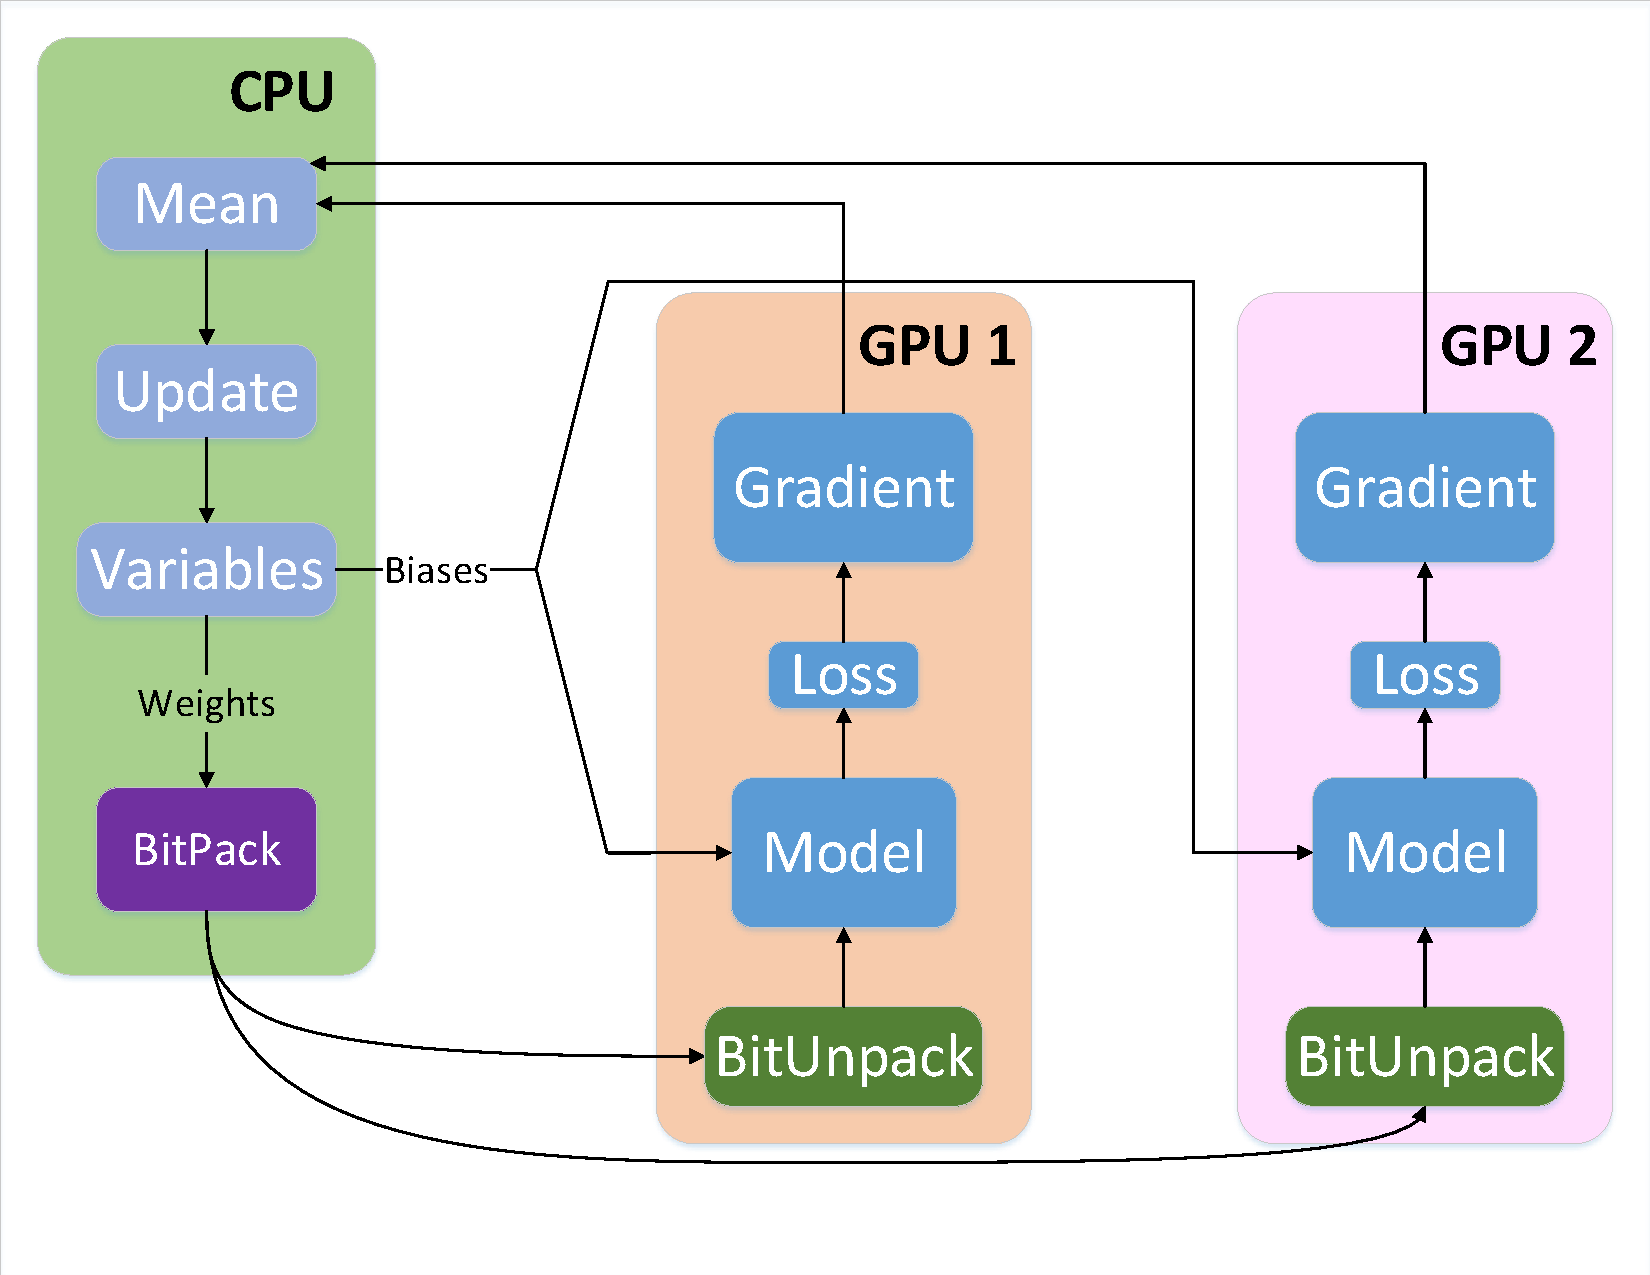
\includegraphics[scale=0.30]{bitpack/figs/tensorflow_multigpu.pdf}}
        \caption{The ADt on a 2-GPU system. Variables include: weights which go through
    the ADt procedure and biases which are sent directly to the GPUs to build the
    network model together with the unpacked weights.}
        \label{bitpack_mgpu}
\end{figure}

The Bitpack operation runs on CPU multicore devices.
To boost Bitpack  
we use OpenMP~\cite{openmp} and 
Single-Instruction Multiple Data (SIMD) intrinsics.
OpenMP is used to run Bitpack on several threads.
The use of SIMD instructions allows Bitpack to operate at the SIMD register level, which
avoids incurring large performance penalties in the process of producing the reduced-size weights.
We implement two versions of Bitpack.
One version uses Intel's AVX2~\cite{avx} instruction set and the other one relies on AltiVec~\cite{Altivec}. 
Bitpack can be implemented on top of any SIMD instruction set architecture supporting simple byte shuffling instructions at the register level.
The Bitunpack procedure runs on the GPUs.

It can be trivially parallelized since each weight is mapped
to a single 32-bit FP variable, which means that GPUs can process a
large amount of weights simultaneously and efficiently build the DNN model.
In fact, Bitunpack incurs negligible overhead as Section~\ref{sec:bitpack_performance} shows.

ADT manipulates the internal representation of network weights by discarding some bits.
We use the standard 32-bit IEEE-754 single-precision Floating Point format
~\cite{ieee754} (1 bit sign, 8 bits exponent and 23 bits mantissa) for all the computation routines.
The Bitpack method considers network weights as 32-bit 
words where rounding to $N$ bits means discarding the lowest $32-N$ bits.

\begin{algorithm}%[H]%algorithm* occupies full page
\caption{High Level Pseudo-code Version of Bitpack}
\label{alg:bitpack_na\"{i}ve}
{\fontsize{11}{11}\selectfont
\begin{algorithmic}[1]
    \State W
    \Comment Array of 32-bit Floating Point values containing weights
    \State Pw
    \Comment Array containing the reduced precision weights
    \State RoundTo
    \Comment Number of bytes to keep per weight
    \State POffset := 0
    \Comment Indicates the current size (in bytes) of Pw
    \For {weight \textbf{in} W}
        \State Pw[POffset : POffset+RoundTo] := weight[0 : RoundTo]
        \Comment Copy most significant RoundTo bytes to Pw
        \State POffset := POffset + RoundTo
    \EndFor
\end{algorithmic}
}
\end{algorithm}


\subsection{Bitpack}
\label{subsec:bitpack}
A high-level version of the Bitpack procedure in terms of pseudo-code is illustrated by 
Algorithm~\ref{alg:bitpack_na\"{i}ve}.
The algorithm requires a couple of arrays: the input array $W$, which contains all the weights of a certain network layer, and an 
output array $Pw$, which stores the compressed versions of these weights. 
The algorithm goes through 
the entire $W$ input array, per each weight, copies the most 
significant $RoundTo$ bytes to the output array $Pw$.
Our Bitpack implementation manipulates data at the byte granularity.
We do not observe significant performance benefits when operating at finer granularity in the experiments we run.
The AWP algorithm described in Section~\ref{sec:bitpack_adaptive} determines the data representation format per each network layer.  
The number of bits of the chosen format is rounded to the nearest number of bytes
that retains all of its information (E.g., if AWP provides the value 14, $RoundTo$ will be set to 2 bytes).
The $Pw$ array is sent to the GPUs once the Bitpack procedure finishes compressing network weights.
%Currently, the host (CPU) and device (GPU) transfer byte stream so a packing
%algorithm with a granularity beyond one byte (8-bit) incurs more complexity and
%has little impact on the communication footprint. Hence, all the bitpack
%algorithm variants we are going to introduce below have a granularity of one byte.

Deep networks usually contain tens or even hundreds of millions of 
weights~\cite{alexnet, alexnet2, vgg}, which makes any trivial implementation 
of Algorithm~\ref{alg:bitpack_na\"{i}ve} not applicable in practice.
We mitigate compression costs by observing that Algorithm~\ref{alg:bitpack_na\"{i}ve} is trivially parallel since processing one weight just requires the $RoundTo$ parameter.
Algorithm~\ref{alg:bitpack_omp} shows how to parallelize the Bitpack procedure by using OpenMP threads.
Each thread takes care of a certain portion of the array storing network weights.

\begin{algorithm}%[H]%algorithm* occupies full page
\caption{Bitpack with OpenMP}
\label{alg:bitpack_omp}
{\fontsize{11}{11}\selectfont
\begin{algorithmic}[1]
    \State W 
    \Comment Array of 32-bit Floating Point values containing weights
    \State Pw
    \Comment Array containing the reduced precision weights
    \State RoundTo 
    \Comment Number of bytes to keep per weight 
    \State NumThreads
    \Comment Number of OpenMP threads
    \State \textcolor{orange} {\#pragma omp parallel for} %public(Weights, Pweights, RoundTo, workload) 
%    \Comment Distribute a portion of weights W and Pw across OpenMP processes
      \For {weight \textbf{in} W}
            \State POffset := Corresponding position in Pw
            \State Pw[POffset : POffset+RoundTo] := weight[0 : RoundTo]
            \Comment Copy the most significant RoundTo bytes to Pw
      \EndFor
\end{algorithmic}
}
\end{algorithm}

\subsection{Single Instruction Multiple Data Bitpack}
Since all weights within one layer are processed in the same way by the Bitpack procedure, we can leverage Single Instruction Multiple Data (SIMD) instructions to vectorize it.
Most state-of-the-art architectures implement SIMD instruction set: IBM's 
AltiVec~\cite{Altivec}, Intel's Advanced Vector Extensions (AVX)~\cite{avx}, and ARM's Neon~\cite{neon}.
In our experiments we use
Intel's AVX2~\cite{avx}, which implements a set of SIMD 
instructions operating over 256-bit registers, and IBM's AltiVec instruction 
set~\cite{Altivec}, which has SIMD instructions operating over 128-bit registers.
Section~\ref{sec:bitpack_setup} describes the specific details of our evaluation considering both x86 and POWER architectures.
%There are also a set of intrinsic C/C++ that expose the AVX2 instructions to the software stack.  
%Intel provides a set of intrinsics for programming using the 
%SIMD instructions in C/C++, we henceforth will refer to the intrinsics rather than the 
%actual instructions.

Figure~\ref{bitpack_avx2} shows the byte-level operations of SIMD-based Bitpack applied to eight 32-bit weights and implemented with AVX2. 
The \textit{RoundTo} parameter is set to 3, which implies discarding the last 8 bits of 
each weight since the target data representation is 24-bit long. 
First, eight 32-bit Floating Point weights are loaded to a 256-bit register.
%of the 16 
%256-bit AVX2 registers. 
In the next step, we use \textit{\_mm256\_shuffle\_epi8} to shuffle the least significant
eight bits of each weight to the least significant bits of their respective 128-bit lane 
(see the grey area of Figure~\ref{bitpack_avx2} Step 2) and pack the rest of the bits 
together. 
Afterwards we use \textit{\_mm256\_permutevar8x32\_epi32} to do the same operation 
across the two 128-bit lanes. 
Finally, we use \textit{\_mm256\_maskstore\_epi32} to just store  
the resulting 192 bits to the target array.
Not all AVX2 instructions operate over the entire 256-bit register.
Instead, many of
them conceive the register as two 128-bit lanes and operate on them separately.
This is the reason way we can not carry out Steps 2 and 3 by using a single AVX2 instruction.


\definecolor{lightgray}{gray}{0.5}
\begin{figure}[H]%[bhtp]
    \centering
    \begin{bytefield}[bitwidth=1.15em, bitformatting={\tiny},endianness=big]{32}
        \wordbox{2}{\textit{\fontsize{11}{11} \selectfont 
            Step 1: Load 8 32-bit weights into a 256-bit AVX2 register. 
            \textcolor{cyan}{(\_mm256\_loadu\_si256)}}} \\ 
        \bitboxes{4}{{\tiny $H_{3..0}$}&{\tiny $G_{3..0}$}&{\tiny $F_{3..0}$}&
                    {\tiny $E_{3..0}$}&{\tiny $D_{3..0}$}&
                    {\tiny $C_{3..0}$}&{\tiny $B_{3..0}$}&{\tiny $A_{3..0}$}} \\
        \bitheader{0,3,7,11,15,19,23,27,31} \\
        \wordbox{2}{\textit{\fontsize{11}{11} \selectfont
            Step 2: Pack weights on the 2 128-bit lanes.
            \textcolor{cyan}{(\_mm256\_shuffle\_epi8)}}} \\
        \bitboxes{3}{{\tiny $H_{3..1}$}} & 
        \bitboxes{3}{{\tiny $G_{3..1}$}} & 
        \bitboxes{3}{{\tiny $F_{3..1}$}} & 
        \bitboxes{3}{{\tiny $E_{3..1}$}} & 
        \bitbox{4}{\color{lightgray}\rule{\width}{\height}} &
        \bitboxes{3}{{\tiny $D_{3..1}$}} &
        \bitboxes{3}{{\tiny $C_{3..1}$}} &
        \bitboxes{3}{{\tiny $B_{3..1}$}} &
        \bitboxes{3}{{\tiny $A_{3..1}$}} &
        \bitbox{4}{\color{lightgray}\rule{\width}{\height}} \\
        \bitheader{0,3,6,9,12,15,19,22,25,28,31} \\
        \wordbox{2}{\textit{\fontsize{11}{11} \selectfont
            Step 3: Pack the 8 weights together by rearranging 32-bit across 
            128-lanes.
            \textcolor{cyan}{(\_mm256\_permutevar8x32\_epi32)}}} \\
        \bitboxes{3}{{\tiny $H_{3..1}$}} & 
        \bitboxes{3}{{\tiny $G_{3..1}$}} & 
        \bitboxes{3}{{\tiny $F_{3..1}$}} & 
        \bitboxes{3}{{\tiny $E_{3..1}$}} & 
        \bitboxes{3}{{\tiny $D_{3..1}$}} &
        \bitboxes{3}{{\tiny $C_{3..1}$}} &
        \bitboxes{3}{{\tiny $B_{3..1}$}} &
        \bitboxes{3}{{\tiny $A_{3..1}$}} &
        \bitbox{8}{\color{lightgray}\rule{\width}{\height}} \\
        \bitheader{0, 7, 10, 13, 16, 19, 22, 25, 28, 31} \\
        \wordbox{2}{\textit{\fontsize{11}{11} \selectfont
            Step 4: Store the most significant 24 bytes (192 bits) of data into 
            the target array. \textcolor{cyan}{(\_mm256\_maskstore\_epi32)}}} \\
    \end{bytefield}
	\vspace{-0.5cm}
	\caption{Bitpack implemented with AVX2, RoundTo=3}
	\label{bitpack_avx2}
\end{figure}

%Algorithm~\ref{alg:bitpack_omp_avx} summarizes our implementation of the Bitpack procedure with AVX2.
%It exploits two-level parallelism: first, the input array of weights is distributed across several threads.
%Second, within each thread, the compression of each eight 32-bit weights subset is performed at the register level by means of byte shuffling instructions.  
%This sophisticated procedure exploiting parallelism at both thread and SIMD register levels uses all the available hardware at the multicore level and avoids costly memory accesses.

\begin{algorithm}%[H]%algorithm* occupies full page
\caption{Bitpack with OpenMP + AVX2}
\label{alg:bitpack_omp_avx}
{\fontsize{11}{11}\selectfont
\begin{algorithmic}[1]
    \State W
    \Comment Array of 32-bit Floating Point values containing weights
    \State Pw
    \Comment Array containing the reduced precision weights
    \State RoundTo
    \Comment Number of bytes to keep per weight
    \State \textcolor{orange} {\#pragma omp parallel for} %public(Weights, Pweights, RoundTo, workload) 
%    \For {process := 0 \ldots NumProcesses}
%        \State Distribute a portion of weights W and Pw across OpenMP processes
    \For {weights \textbf{in} W}
        \State \textcolor{cyan}{\_mm256\_loadu\_si256}
        \Comment Load 8 32-bit weights 
        \State \textcolor{cyan}{\_mm256\_shuffle\_epi8}
        \Comment Compress at each 128-bit lane
        \State \textcolor{cyan}{\_mm256\_permutevar8x32\_epi32}
        \Comment Shuffle the compressed weights into the most significant bits
        \State \textcolor{cyan}{\_mm256\_maskstore\_epi32}
        \Comment Store compressed weights to the target array
    \EndFor
\end{algorithmic}
}
\end{algorithm}

\begin{algorithm}%[H]%algorithm* occupies full page
\caption{Bitunpack on GPU}
\label{alg:bitunpack}
{\fontsize{11}{11}\selectfont
\begin{algorithmic}[1]
    \State Pw
    \Comment Array containing compressed weights
    \State W
    \Comment Array of 32-bit Floating Point values containing weights
    \State RoundTo
    \Comment The number of bytes that are going to be kept
    \For{UnitId := 0 \ldots NumUnit}
    \State Distribute W and Pw across all the computation units in the GPU
        \State POffset := 0
        \For{weight in W}
            \State weight := Pw[POffset : POffset+RoundTo] $\ll$ (4 - RoundTo) * 8
            \State POffset := POffset + RoundTo
        \EndFor
    \EndFor
\end{algorithmic}
}
\end{algorithm}

Algorithm~\ref{alg:bitpack_omp_avx} summarizes our implementation of the Bitpack procedure with AVX2.
It exploits two-level parallelism: first, the input array of weights is distributed across several threads.
Second, within each thread, the compression of each eight 32-bit weights subset is performed at the register level by means of byte shuffling instructions.
This sophisticated procedure exploiting parallelism at both thread and SIMD register levels uses all the available hardware and avoids costly memory accesses.

\subsection{Bitunpack}
Once data in reduced-size format reaches the target GPU, the Bitunpack procedure immediately 
restores them into their original IEEE-754 32-bit Floating Point format. 
We display pseudo-code describing this process in Algorithm~\ref{alg:bitunpack}.
Bitunpack reads the reduced-sized weights from array $Pw$ and assigns additional bits to them. 
Bitunpack gives zero values to these additional bits.
We distribute the Bitunpack process across the whole GPU, which enables an extremely parallel scheme exploiting GPUs manycore architecture. 

The Bitunpack routine is developed using CUDA~\cite{cuda}. 
Our code  
runs in parallel on $N$ CUDA threads and the CUDA runtime handles the dynamic mapping between threads and the underlying GPU compute units.
Since each thread involved in the parallel run targets a different portion of the $Pw$ array, our Bitunpack procedure exposes a large amount of parallelism able to exploit the large number of compute units integrated into high-end GPU devices.

